\documentclass[10pt,landscape]{article}
\usepackage[letterpaper,landscape,margin=0.43in]{geometry}
\usepackage{amsmath,amssymb}
\usepackage[T1]{fontenc}
\usepackage{lmodern}
\usepackage{xcolor}
\usepackage{tikz}
\usepackage{graphicx}
\usetikzlibrary{arrows.meta,positioning,calc,fit,backgrounds,shapes.geometric}
\usepackage{listings}
\pagestyle{empty}
\setlength{\parindent}{0pt}

\definecolor{ink}{HTML}{172033}
\definecolor{muted}{HTML}{637083}
\definecolor{blue}{HTML}{2563EB}
\definecolor{bluepale}{HTML}{EAF2FF}
\definecolor{teal}{HTML}{0F8B8D}
\definecolor{tealpale}{HTML}{E6F7F5}
\definecolor{amber}{HTML}{D97706}
\definecolor{amberpale}{HTML}{FFF4D6}
\definecolor{violet}{HTML}{7C3AED}
\definecolor{violetpale}{HTML}{F2EAFF}
\definecolor{green}{HTML}{16825D}
\definecolor{greenpale}{HTML}{E7F7EF}
\definecolor{linegray}{HTML}{CBD5E1}

\tikzset{
  >={Stealth[length=2.2mm,width=1.5mm]},
  card/.style={draw=linegray, rounded corners=3mm, fill=white, line width=.65pt},
  pill/.style={rounded corners=2mm, inner xsep=3mm, inner ysep=1.4mm, font=\bfseries\small},
  flow/.style={->, line width=1.1pt, color=muted},
  tinyflow/.style={->, line width=.85pt, color=muted},
  dot/.style={circle, minimum size=3.2mm, inner sep=0pt}
}

\lstdefinelanguage{Lean}{
  morekeywords={theorem,namespace,end,by,convert,Set,Type},
  sensitive=true,
  morecomment=[l]{--},
  morestring=[b]"
}
\lstset{language=Lean,basicstyle=\ttfamily\small,keywordstyle=\color{violet}\bfseries,
  commentstyle=\color{muted},showstringspaces=false,columns=fullflexible,keepspaces=true}

\newcommand{\Title}[2]{%
  {\fontsize{22}{24}\selectfont\bfseries\color{ink}#1}\hfill
  \tikz[baseline=-.6ex]\node[pill,fill=#2!12,text=#2]{PROOF REUSE};
  \par\vspace{1mm}\color{linegray}\rule{\linewidth}{0.8pt}\color{ink}\vspace{2mm}}
\newcommand{\Tag}[2]{\tikz[baseline=-.6ex]\node[pill,fill=#1,text=#2]{#2};}

\begin{document}
\color{ink}

% PAGE 1
\Title{One proof, hiding in three places}{blue}

\begin{minipage}[t]{0.31\linewidth}
\resizebox{\linewidth}{!}{%
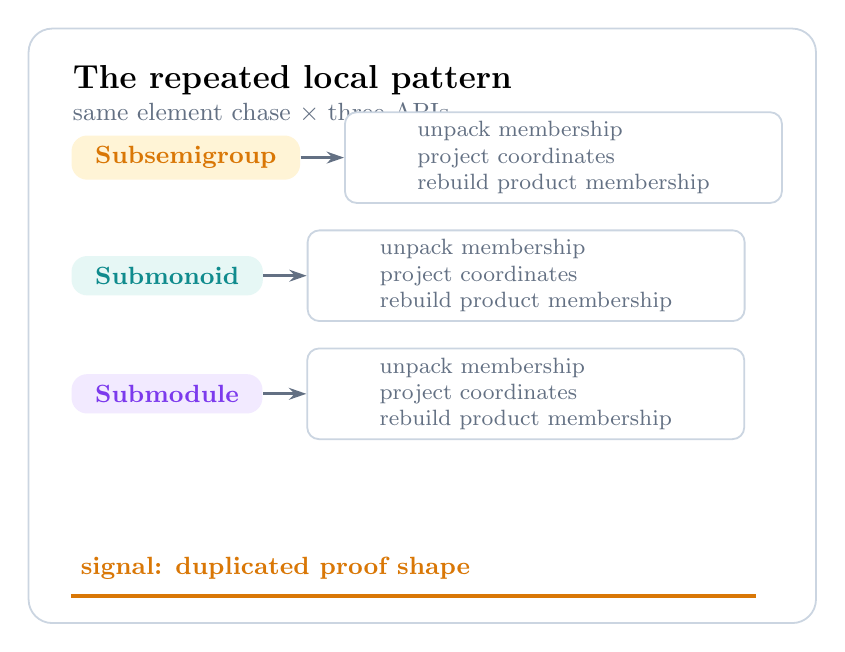
\begin{tikzpicture}[x=1cm,y=1cm]
  \node[card,minimum width=10.0cm,minimum height=7.55cm,anchor=north west] (c) at (0,0) {};
  \node[anchor=north west,font=\bfseries\large] at (.45,-.35) {The repeated local pattern};
  \node[anchor=north west,text=muted,font=\small] at (.45,-.84) {same element chase $\times$ three APIs};

  \node[pill,fill=amberpale,text=amber,anchor=west] (sg) at (.55,-1.65) {Subsemigroup};
  \node[pill,fill=tealpale,text=teal,anchor=west] (sm) at (.55,-3.15) {Submonoid};
  \node[pill,fill=violetpale,text=violet,anchor=west] (su) at (.55,-4.65) {Submodule};

  \foreach \n/\y in {sg/-1.65,sm/-3.15,su/-4.65}{
    \draw[flow] (\n.east) -- ++(.55,0) node[right,card,rounded corners=1.5mm,
      minimum width=5.55cm,minimum height=1.02cm,align=left,font=\footnotesize] (x\y)
      {unpack membership\\project coordinates\\rebuild product membership};
  }
  \node[anchor=south west,font=\bfseries\small,text=amber] at (.55,-7.13) {signal: duplicated proof shape};
  \draw[amber,line width=1.6pt] (.55,-7.22) -- (9.25,-7.22);
\end{tikzpicture}}
\end{minipage}\hfill
\begin{minipage}[t]{0.655\linewidth}
\resizebox{\linewidth}{!}{%
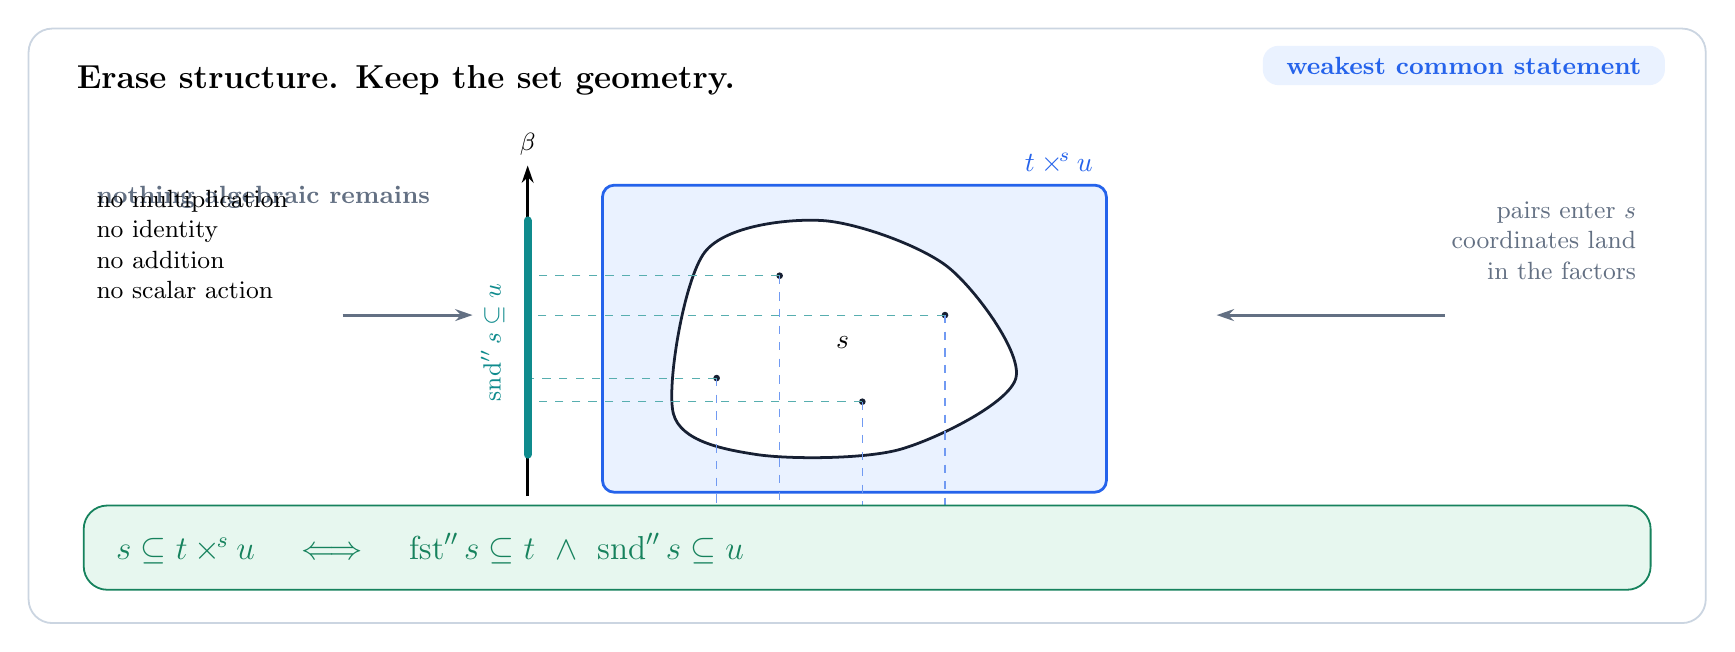
\begin{tikzpicture}[x=1cm,y=1cm]
  \node[card,minimum width=21.3cm,minimum height=7.55cm,anchor=north west] (c) at (0,0) {};
  \node[anchor=north west,font=\bfseries\large] at (.5,-.35) {Erase structure. Keep the set geometry.};
  \node[pill,fill=bluepale,text=blue,anchor=east] at (20.8,-.48) {weakest common statement};

  % product rectangle
  \draw[rounded corners=1.5mm,fill=bluepale,draw=blue,line width=1pt] (7.3,-2.0) rectangle (13.7,-5.9);
  \node[anchor=south east,text=blue,font=\bfseries] at (13.65,-1.98) {$t\times^{\!s}u$};
  \draw[fill=white,draw=ink,line width=1pt,smooth cycle]
    plot coordinates {(8.2,-4.9) (8.6,-2.85) (10.1,-2.45) (11.7,-3.05) (12.55,-4.45) (11.1,-5.35) (9.25,-5.42)};
  \node[font=\bfseries] at (10.35,-4.0) {$s$};
  \foreach \x/\y in {8.75/-4.45,9.55/-3.15,10.6/-4.75,11.65/-3.65}{
    \fill[ink] (\x,\y) circle (1.2pt);
    \draw[blue!65,dashed] (\x,\y)--(\x,-6.45);
    \draw[teal!70,dashed] (\x,\y)--(6.35,\y);
  }
  \draw[->,line width=1pt] (7.2,-6.45)--(13.9,-6.45) node[right,font=\small] {$\alpha$};
  \draw[->,line width=1pt] (6.35,-5.95)--(6.35,-1.75) node[above,font=\small] {$\beta$};
  \draw[blue,line width=3pt,line cap=round] (8.2,-6.45)--(12.6,-6.45);
  \draw[teal,line width=3pt,line cap=round] (6.35,-5.42)--(6.35,-2.45);
  \node[text=blue,font=\bfseries\small,below] at (10.4,-6.5) {$\operatorname{fst}''s\subseteq t$};
  \node[text=teal,font=\bfseries\small,rotate=90,above] at (6.18,-4.0) {$\operatorname{snd}''s\subseteq u$};

  \node[card,fill=greenpale,draw=green,minimum width=19.9cm,minimum height=1.07cm,
    anchor=south west] at (.7,-7.15) {};
  \node[anchor=west,text=green,font=\bfseries\large] at (1.0,-6.62)
    {$s\subseteq t\times^{\!s}u\quad\Longleftrightarrow\quad
      \operatorname{fst}''s\subseteq t\ \wedge\ \operatorname{snd}''s\subseteq u$};

  \node[anchor=west,font=\bfseries\small,text=muted] at (.75,-2.15) {nothing algebraic remains};
  \node[anchor=west,align=left,font=\small] at (.75,-2.75)
    {no multiplication\\no identity\\no addition\\no scalar action};
  \draw[flow] (4.0,-3.65) -- (5.65,-3.65);

  \node[anchor=east,align=right,font=\small,text=muted] at (20.55,-2.7)
    {pairs enter $s$\\coordinates land\\in the factors};
  \draw[flow] (18.0,-3.65) -- (15.1,-3.65);
\end{tikzpicture}}
\end{minipage}

\vfill

\begin{tikzpicture}
  \node[pill,fill=ink,text=white] {BIG IDEA};
  \node[anchor=west,font=\bfseries\large] at (2.75,0)
    {When proofs repeat below different structures, descend to the common carrier.};
\end{tikzpicture}

\newpage

% PAGE 2
\Title{The generic lemma becomes a proof junction}{teal}

\begin{minipage}[t]{0.58\linewidth}
\resizebox{\linewidth}{!}{%
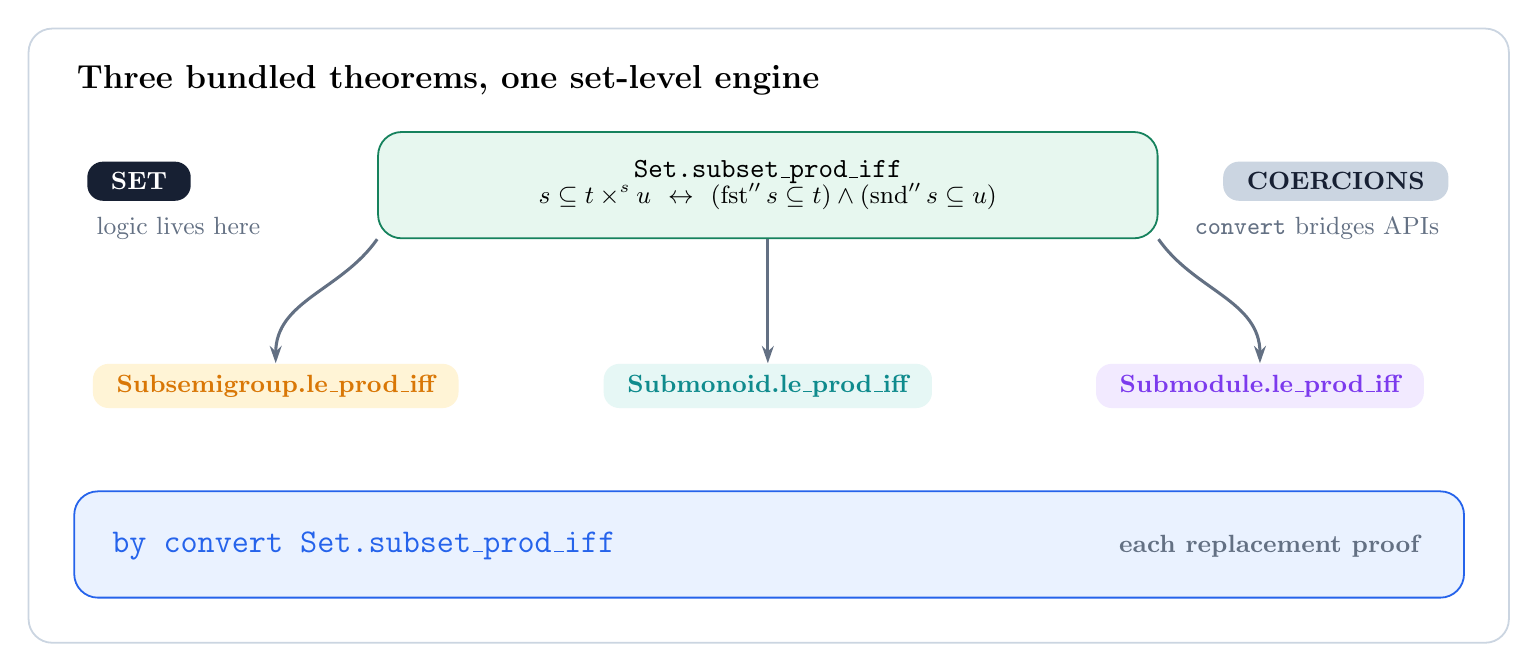
\begin{tikzpicture}[x=1cm,y=1cm]
  \node[card,minimum width=18.8cm,minimum height=7.8cm,anchor=north west] at (0,0) {};
  \node[anchor=north west,font=\bfseries\large] at (.5,-.35) {Three bundled theorems, one set-level engine};

  \node[card,fill=greenpale,draw=green,minimum width=9.9cm,minimum height=1.35cm,
    align=center,font=\bfseries] (core) at (9.4,-2.0)
    {\texttt{Set.subset\_prod\_iff}\\[-1mm]
     \small $s\subseteq t\times^{s}u\ \leftrightarrow\
     (\operatorname{fst}''s\subseteq t)\wedge(\operatorname{snd}''s\subseteq u)$};

  \node[pill,fill=amberpale,text=amber] (a) at (3.15,-4.55) {Subsemigroup.le\_prod\_iff};
  \node[pill,fill=tealpale,text=teal] (b) at (9.4,-4.55) {Submonoid.le\_prod\_iff};
  \node[pill,fill=violetpale,text=violet] (d) at (15.65,-4.55) {Submodule.le\_prod\_iff};
  \draw[flow] (core.south west) to[out=235,in=90] (a.north);
  \draw[flow] (core.south) -- (b.north);
  \draw[flow] (core.south east) to[out=305,in=90] (d.north);

  \node[card,fill=bluepale,draw=blue,minimum width=17.65cm,minimum height=1.35cm,
    anchor=south west] at (.58,-7.25) {};
  \node[anchor=west,font=\ttfamily\large,text=blue] at (.95,-6.58)
    {by  convert Set.subset\_prod\_iff};
  \node[anchor=east,font=\bfseries\small,text=muted] at (17.8,-6.58)
    {each replacement proof};

  \node[pill,fill=ink,text=white,anchor=west] at (.75,-1.95) {SET};
  \node[anchor=west,font=\small,text=muted] at (.75,-2.55) {logic lives here};
  \node[pill,fill=linegray,text=ink,anchor=east] at (18.05,-1.95) {COERCIONS};
  \node[anchor=east,font=\small,text=muted] at (18.05,-2.55) {\texttt{convert} bridges APIs};
\end{tikzpicture}}
\end{minipage}\hfill
\begin{minipage}[t]{0.405\linewidth}
\resizebox{\linewidth}{!}{%
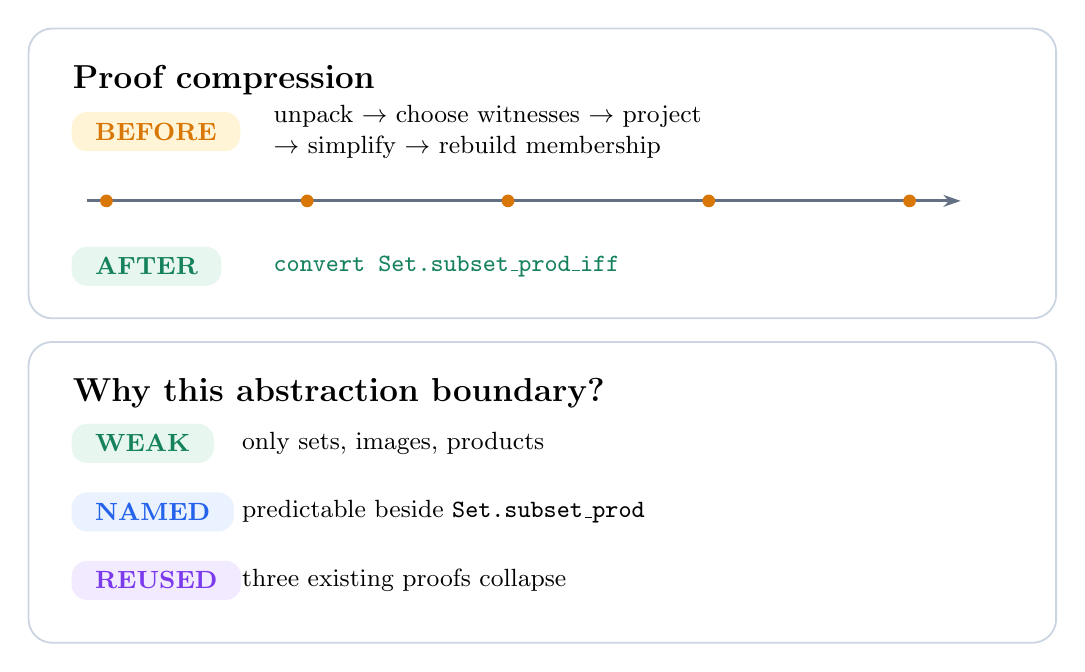
\begin{tikzpicture}[x=1cm,y=1cm]
  \node[card,minimum width=13.05cm,minimum height=3.68cm,anchor=north west] at (0,0) {};
  \node[anchor=north west,font=\bfseries\large] at (.45,-.35) {Proof compression};
  \node[pill,fill=amberpale,text=amber,anchor=west] at (.55,-1.32) {BEFORE};
  \node[anchor=west,font=\small,align=left] at (3.0,-1.32)
    {unpack $\to$ choose witnesses $\to$ project\\$\to$ simplify $\to$ rebuild membership};
  \draw[flow] (.75,-2.2)--(11.85,-2.2);
  \foreach \x in {1.0,3.55,6.1,8.65,11.2}{\fill[amber] (\x,-2.2) circle (2.3pt);}
  \node[pill,fill=greenpale,text=green,anchor=west] at (.55,-3.03) {AFTER};
  \node[anchor=west,font=\ttfamily\small,text=green] at (3.0,-3.03)
    {convert Set.subset\_prod\_iff};

  \node[card,minimum width=13.05cm,minimum height=3.82cm,anchor=north west] at (0,-3.98) {};
  \node[anchor=north west,font=\bfseries\large] at (.45,-4.33) {Why this abstraction boundary?};
  \node[pill,fill=greenpale,text=green,anchor=west] at (.55,-5.28) {WEAK};
  \node[anchor=west,font=\small] at (2.6,-5.28) {only sets, images, products};
  \node[pill,fill=bluepale,text=blue,anchor=west] at (.55,-6.15) {NAMED};
  \node[anchor=west,font=\small] at (2.6,-6.15) {predictable beside \texttt{Set.subset\_prod}};
  \node[pill,fill=violetpale,text=violet,anchor=west] at (.55,-7.02) {REUSED};
  \node[anchor=west,font=\small] at (2.6,-7.02) {three existing proofs collapse};
\end{tikzpicture}}
\end{minipage}

\vfill
\resizebox{\linewidth}{!}{%

\begin{tikzpicture}[x=1cm,y=1cm]
  \node[pill,fill=ink,text=white] (find) {FIND};
  \node[pill,fill=amberpale,text=amber,right=1.25cm of find] (erase) {ERASE STRUCTURE};
  \node[pill,fill=greenpale,text=green,right=1.25cm of erase] (state) {STATE THE CORE};
  \node[pill,fill=bluepale,text=blue,right=1.25cm of state] (reuse) {REUSE BY CONVERSION};
  \draw[flow] (find)--(erase); \draw[flow] (erase)--(state); \draw[flow] (state)--(reuse);
  \node[anchor=east,font=\bfseries\large] at (31.3,0) {duplication $\Rightarrow$ upstream-sized lemma};
\end{tikzpicture}}

\end{document}
